\section{Analysis}
We addressed our two research questions separately.

\subsection{Question 1}
Technically, the data we collected were asymmetric; that is, we have separate data from when group $A$ serves as the target and group $B$ serves as the distracter than when group $A$ serves as the distracter and group $B$ serves as the target. While we suspected this would be a very comparable task, we performed McNemar's test to determine if our data was symmetric.  As it failed standard tests of significance $p > 0.1$, we decided to pool the data. See Figure~\ref{fullacc} for the non-symmetric accuracies.

To determine whether people could naively distinguish among wallpaper groups, we performed binomial t-tests comparing participants' actual performance to chance ($\pi=0.5$). Using this paradigm, we found that $135/136$ tests were significant at the $p<0.05$ level; the last test was still significant at the $p<0.10$ level. We computed t-tests individually to check whether every group was distinguishable from every other, rather than if the average two groups were distinguishable. There was clear variation in these probabilities, although people were able to distinguish among the wallpaper groups significantly better than chance. 

The most difficult pair for participants to distinguish between were P4M and PMM (see Figure~\ref{pmmp4m} for an example). Interestingly, an expert given a small amount of time should have almost no trouble distinguishing them, as the lack of 4-fold rotation is quite obvious in PMM. Across the 96 participants, only 56.8\% of trials were successful. For comparison, the average accuracy among all trials was 76.8\%. However, there remains a possibility that certain groups are nearly indistinguishable to non-experts.

\begin{figure}[!ht]
\centering
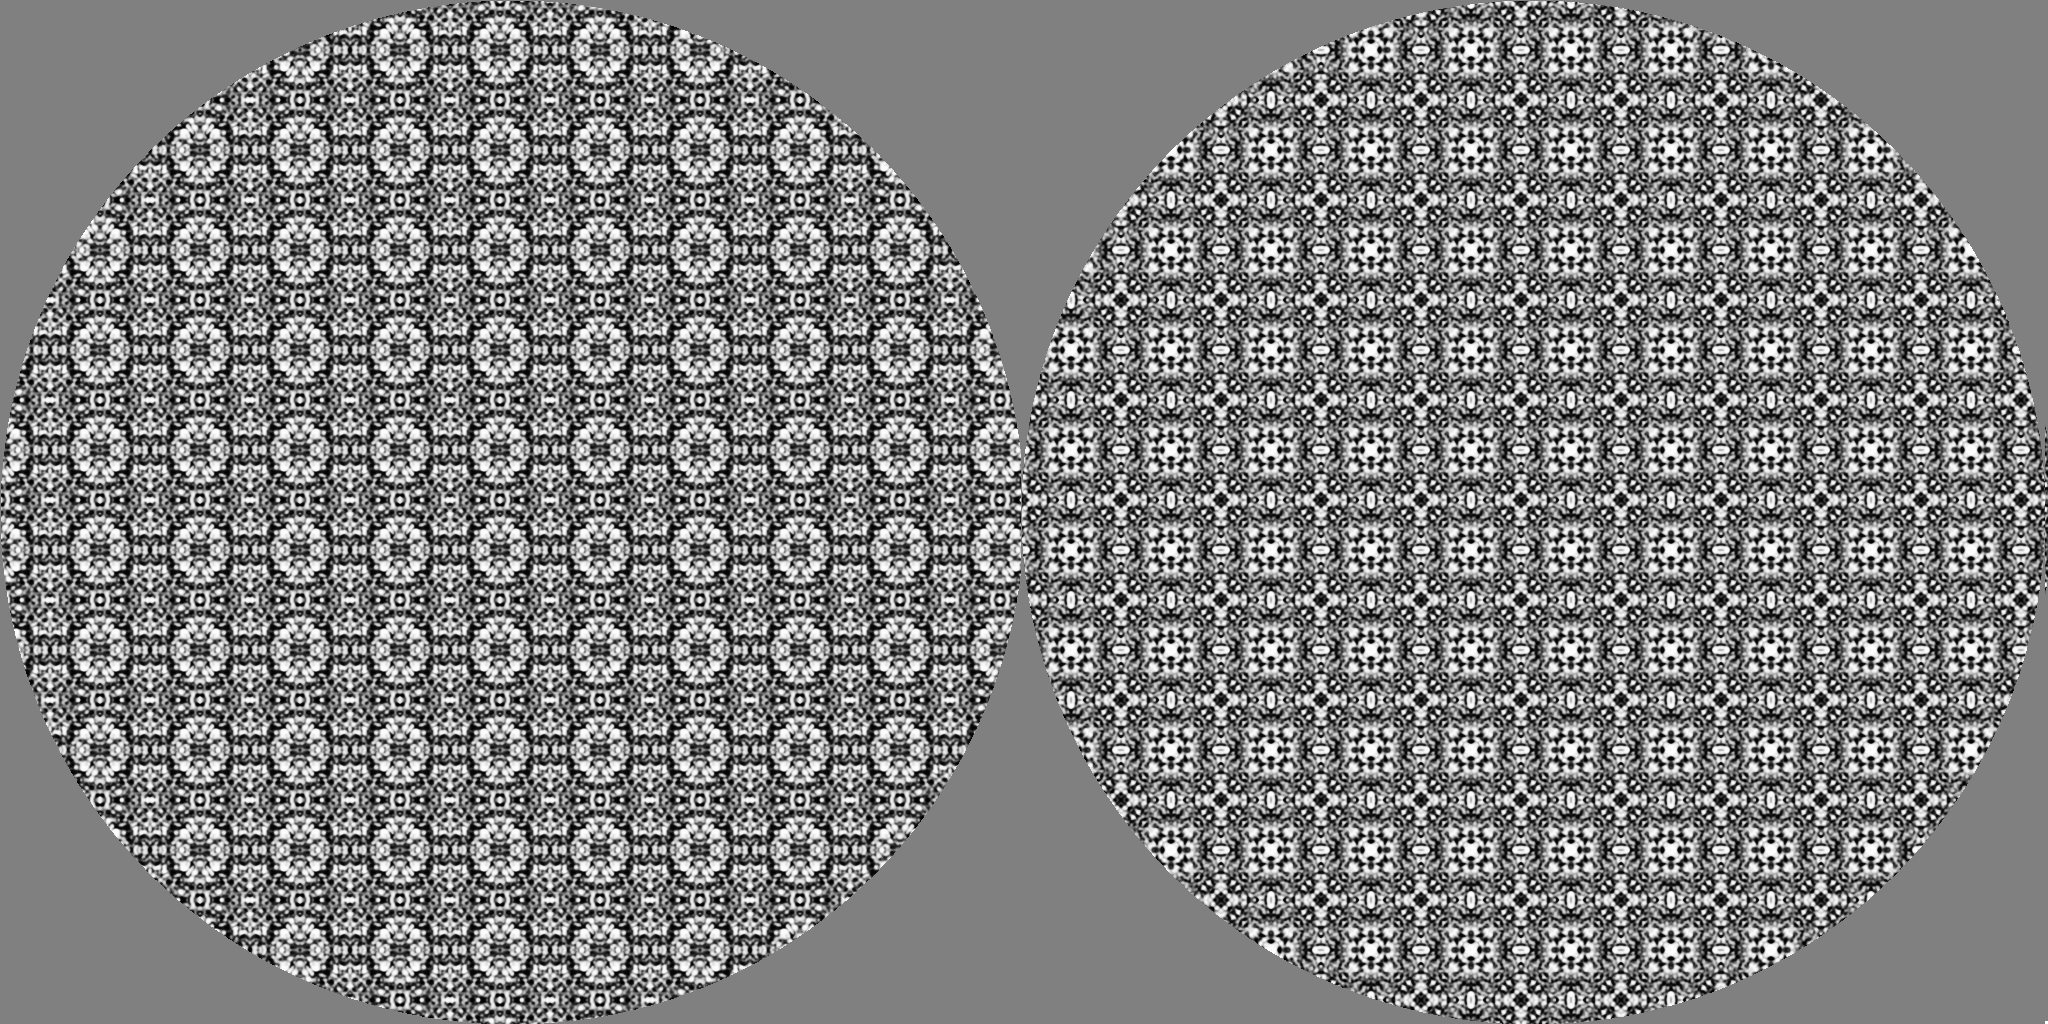
\includegraphics[width=0.9\columnwidth]{pmmp4m}
\caption{PMM on the left (note the tiles lack reflection on the horizontal axis, but have it on the vertical axis), P4M on the right.}
\label{pmmp4m}
\end{figure}

\begin{figure}[!ht]
\centering
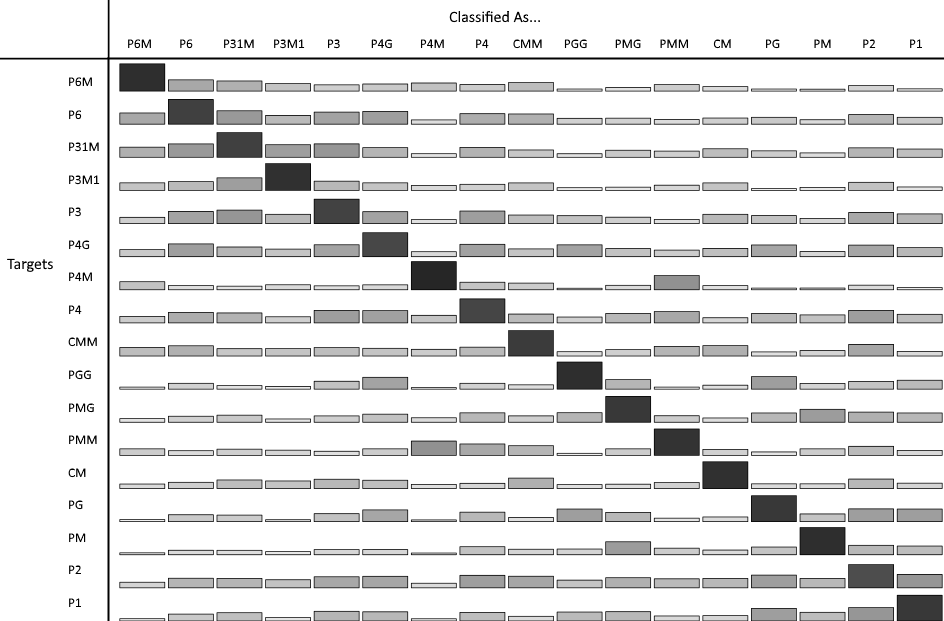
\includegraphics[width=0.9\columnwidth]{accuracies-grayscale}
\caption{On the vertical we have the targets. On the top are the distracters. The bars represent the percentage of errors. The main diagonal, where the target and distracter are the same, represents the aggregate accuracy in labeling that group correctly. The darkness of the bar also corresponds to its value (higher is darker).}
\label{fullacc}
\end{figure}

\subsection{Question 2}
To answer our second question, we used a Linear Mixed Effects Regression (GLMM) model. We tried to determine which symmetries contributed to accuracy. Thus, we used a comparison of each task's symmetries as the model.
\begin{enumerate}
\item 2-Fold Rotation, 3-Fold Rotation, 4-Fold Rotation, 6-Fold Rotation (True, False). In this case, groups with 6-Fold are guaranteed to have 3-Fold and 2-Fold.
\item Reflection, Glide Reflection, or nothing along the four main axes ($T_1, T_2, D_1, D_2$)
\item Tile Shape. This feature is not included in the group-theoretic analysis, but might play a role
\item Subgroup distance, computed with Djikstra's algorithm. 
\end{enumerate}

We included two random effect intercepts grouped by participant and the specific task (combined by-item and by-subject analysis).

% THIS IS TOO MUCH DETAIL FOR A COGSCI PAPER
 % while it would contain the same groups, the group being on the top or bottom might play some small role. While we could have iteratively designed a uniform test set avoiding this issue, random effects allow us to control for the variance our methodology caused.

The best model was identified according to Aikake Information Criterion (AIC), among the models including the pool of features described earlier. This best model included distance, but additionally included the $T_1$ axis, which would correspond to bilateral reflection symmetry, the $D_1$ axis, which is the positive diagonal, 4-fold rotation, and 3-fold rotation. See Table~\ref{fixeff} for the fixed effects in a model including all possible features.